\documentclass[12pt,twoside, letter]{exam}
\usepackage{enumitem, kantlipsum}
\usepackage[margin=1in,left=1in,right=1in,top=1in,bottom=1in]{geometry}
\usepackage{graphicx,epstopdf}
\usepackage{amssymb,amsmath,amsfonts, amsthm}
\usepackage{wasysym}
\newtheorem{theorem}{Theorem}
\newtheorem{corollary}{Corollary}[theorem]
\newtheorem{lemma}[theorem]{Lemma}
\usepackage{hyperref}
\usepackage{tikz}
\usepackage{xstring}
\usetikzlibrary{calc}
\usepackage{ducksay}
\newtheorem{prop}{Proposition}

\theoremstyle{definition}
\newtheorem{definition}{Definition}

\usepackage{bbm}
\usepackage{verbatim}
\usepackage{bbold}
\usepackage{phfparen}
\usepackage{sets}
\newcommand{\nn}{\mathbb{N}}
\newcommand{\rr}{\mathbb{R}}
\newcommand{\cc}{\mathbb{C}}
\newcommand{\cb}{\mathcal{B}}
\newcommand{\ctau}{\mathcal{T}}
\newcommand{\co}{\mathcal{O}}
\newcommand{\zz}{\mathbb{Z}}
\newcommand{\ee}{\mathbb{E}}
\newcommand{\qq}{\mathbb{Q}}
\newcommand{\interior}{\text{Int}}
\newcommand{\pp}{\mathbb{P}}
\newcommand{\id}{\mathbbm{1}}
\newcommand{\Co}{\text{Co}}
\newcommand{\Cl}{\text{Cl}}
\usepackage{mathtools}
\DeclarePairedDelimiter\ceil{\lceil}{\rceil}
\DeclarePairedDelimiter\floor{\lfloor}{\rfloor}


\usepackage{indentfirst}
\setlist{
    listparindent = \parindent,
    parsep = 6pt,
}

\makeatletter
\newsavebox\myboxA
\newsavebox\myboxB
\newlength\mylenA

\newcommand*\xoverline[2][0.9]{%
    \sbox{\myboxA}{$\m@th#2$}%
    \setbox\myboxB\null% Phantom box
    \ht\myboxB=\ht\myboxA%
    \dp\myboxB=\dp\myboxA%
    \wd\myboxB=#1\wd\myboxA% Scale phantom
    \sbox\myboxB{$\m@th\overline{\copy\myboxB}$}%  Overlined phantom
    \setlength\mylenA{\the\wd\myboxA}%   calc width diff
    \addtolength\mylenA{-\the\wd\myboxB}%
    \ifdim\wd\myboxB<\wd\myboxA%
       \rlap{\hskip 0.5\mylenA\usebox\myboxB}{\usebox\myboxA}%
    \else
        \hskip -0.5\mylenA\rlap{\usebox\myboxA}{\hskip 0.5\mylenA\usebox\myboxB}%
    \fi}
\makeatother

\usepackage{float}
\floatstyle{boxed}
\restylefloat{figure}

\printanswers

\begin{document}


\abovedisplayskip=12pt
\belowdisplayskip=12pt
\abovedisplayshortskip=7pt
\belowdisplayshortskip=10pt
\allowdisplaybreaks

\setlength{\parindent}{18pt}

\title{Quantitative Methods: Assignment 2}
\author{Raymond Luo}
\date{\today}
\maketitle

\noindent {\bf Problem 1 (30 points):}
\begin{enumerate}
  \item Write a program to implement a symmetric random walk $X_{n}$ of $n$ steps, starting at $X_0 = 0$, using a random number generator to choose the
    direction of each step. Provide a printout of your code.
  \item Run your program for $N = 10,000$
  \item Plot $X_n$ as a function of $n$, for $0 \leq n \leq N$.
  \item Set
    \begin{equation*}
      W_{n} = \frac{1}{\sqrt{n}} X_{n}
    \end{equation*}
    Plot $W_n$ as a function of $n$, for $0 \leq n \leq N$.
\end{enumerate}

  We have the following code:
  \\
  \begin{figure}[h]
    \centering
        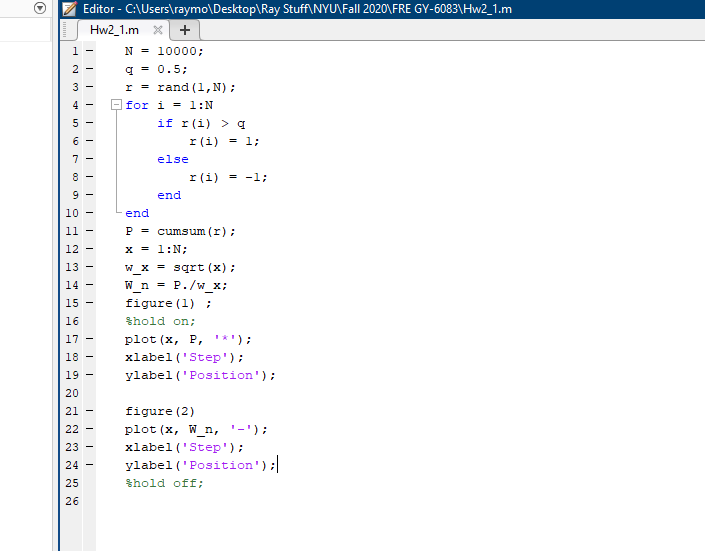
\includegraphics[width=4in]{Hw2_1c}
  \end{figure}
  \\
  From which we produce the following random walk (zoomed out):
  \\
  \begin{figure}[h]
    \caption{$X_{n}$}
    \centering
      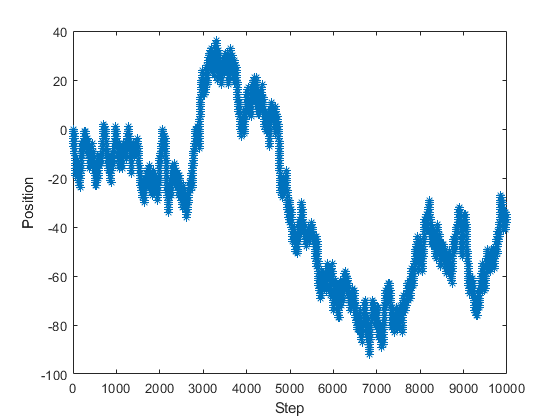
\includegraphics[width=3in]{Hw2_1a}
  \end{figure}
  \\
  And we get the following $W_{n}$ as a function of $n$:
  \\
  \begin{figure}[h]
    \caption{$W_{n}$}
    \centering
      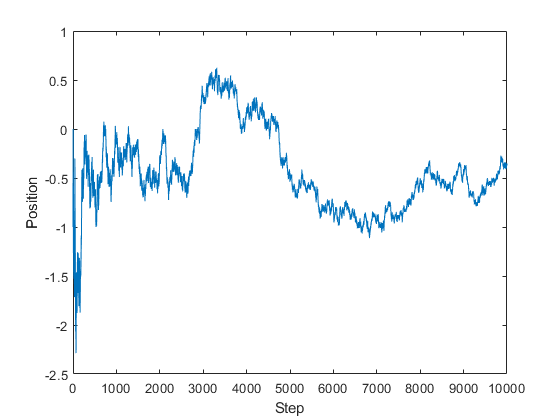
\includegraphics[width=3in]{Hw2_1b}
  \end{figure}



\noindent {\bf Problem 2 (30 points):}
\par{Consider a random walk which is not necessarily symmetric, where the probability of a head is given by $p \in (0,1)$, where as the probability of a tail is $q = 1-p$.
As you know, the random is walk is not necessarily a martingale}

\begin{enumerate}
  \item What is the expectation of the random walk for $p = 0.3$?
    \begin{solution}
      $\forall i \in \nn, \ee[X_{i}] = 1\cdot p + (-1) \cdot q = 0.3 - 0.7 = -0.4$. It then follows that $\lim_{n \rightarrow \infty} \ee[S_{n}] \\
      = \lim_{n \rightarrow \infty} \ee[\sum_{i=1}^n X_{i}] = \lim_{n \rightarrow \infty} \sum_{i=1}^n \ee[X_{i}] =\sum^{\infty}_{i=1} -0.4 = -\infty$.
    \end{solution}
  \item Plot a sample path of the random walk corresponding to $p = 0.3$ for $N = 10,000$ steps. \\
    Solution:
      \begin{figure}[h]
        \caption{$X_{n}$ with $p = 0.3$}
        \centering
          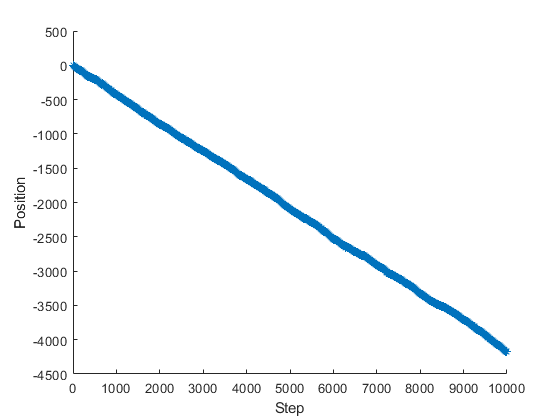
\includegraphics[width=3in]{Hw2_1d}
      \end{figure}
  \item Does this random walk have a tendency to go up for down?
    \begin{solution}
      This random walk has a tendency to go down.
    \end{solution}
  \item Answer the previous 3 questions for a random walk corresponding to $p = 0.7$\\
    Solution:\\
    \\
        i) $\forall i \in \nn, \ee[X_{i}] = 1\cdot p + (-1) \cdot q = 0.7 - 0.3 = 0.4$. It then follows that $\lim_{n \rightarrow \infty} \ee[S_{n}] \\
        = \lim_{n \rightarrow \infty} \ee[\sum_{i=1}^n X_{i}] = \lim_{n \rightarrow \infty} \sum_{i=1}^n \ee[X_{i}] =\sum^{\infty}_{i=1} 0.4 = +\infty$. \\
        ii) \\
          \begin{figure}[h]
            \caption{$X_{n}$ with $p = 0.7$}
            \centering
              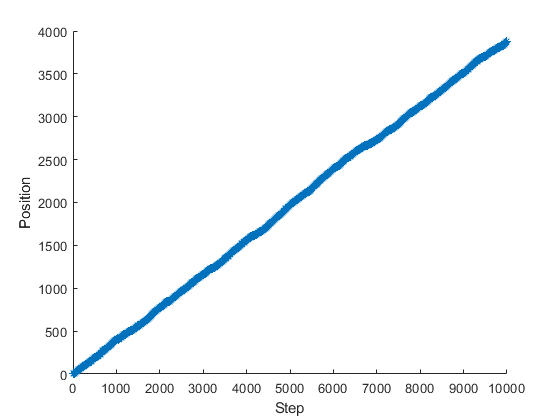
\includegraphics[width=3in]{Hw2_1e}
          \end{figure}
        iii) This random walk has a tendency to go up.
\end{enumerate}


\noindent {\bf Problem 3 (25 points):}
\par{Consider the integral}
  \begin{equation*}
    a = \int^1_0 f(x) dx
  \end{equation*}
It can be interpreted as the following expectation
  \begin{equation*}
    \ee[f(U)]
  \end{equation*}
where U is a random variable that is uniformly distributed on the interval (0,1). Consider next a sequence $U_1, U_2, \cdots, U_n$ of independent and uniformly distributed
random variables in the interval (0,1).

\begin{enumerate}
  \item Show that
    \begin{equation*}
      \lim_{n \rightarrow +\infty} \frac{1}{n} \sum^n_{i=1} f(U_{i}) = a, \text{ almost surely }.
    \end{equation*}

    \begin{solution}
      This follows directly from the Strong Law of Large Numbers, as \\
      $\lim_{n \rightarrow +\infty} \frac{1}{n} \sum^n_{i=1} f(U_{i}) = \ee[f(U)] = \int^1_0 f(x) d(U(X)) = \int^1_0 f(x) dx = a$.
    \end{solution}

  \item What is the distribution of the error
    \begin{equation*}
      \frac{1}{n} \sum^{n}_{i = 1} f(U_{i}) - a?
    \end{equation*}

    \begin{solution}
      We note that as $\{U_i\}_{i\in\nn}$ is a sequence of random variables, $\{f(U_i)\}_{i\in\nn}$ is also a sequence of random variables (as it maps the measurable codomain space of $f$ to
      another measurable subspace of $\rr$). We also observe that $\ee[f(U)] = a$ implies that $f(U)$ has finite expectation. If we suppose that $f(U)$ has some finite variance $\sigma^{2}$, by
      the central limit theorem, we have that $\frac{1}{n} \sum^{n}_{i = 1} f(U_{i})$ converges in distribution to a normal distribution with mean $a = \ee[f(U)]$ and variance $\sigma^{2}/n$.
      It then follows that the error is convergent in distribution to a normal distribution.
    \end{solution}

\end{enumerate}

\noindent {\bf Problem 4 (15 points):}
\par{Let $\{X_{n}, n = 1,2, \cdots \}$ be a discrete-time and discrete-state stochastic process such that, for every $n, i, j$ and every $i_1, \cdots i_{n-1}$,}
\begin{equation*}
  \pp[X_{n+1} = j \mid X_n = i, X_{n-1} = i_{n-1}, \cdots, X_{1} = i_1] = \pp[X_{n+1} = j \mid X_{n} = i, X_{n-1}=i_{n-1}]
\end{equation*}

\begin{enumerate}
  \item Is this process Markovian? Explain.
    \begin{solution}
      No, we are observing a Markov chain of order 2 which is not Markovian in the usual sense as it depends on the observation of two previous states as opposed to the last state.
    \end{solution}
  \item Can you make it Markovian by modifying it slightly? In other words, can you define another Markov process $(Y_{n})$ which is based on $X_{n}$ but whose definition differs slightly
  from the definition of $(X_{n})$ and which satisfies the Markov property? IF this is possible, give the definition of $(Y_{n})$ and show that $(Y_{n})$ is Markovian.
    \begin{solution}
      We can define $Y_{n} = (X_{n}, X_{n-1})$ to satisfy the Markov property. We note that:
        \begin{multline*}
          \pp[Y_{n+1} = j_{n+1} \mid X_n = i, X_{n-1} = i_{n-1}, \cdots, X_{1} = i_1] \\
          = \pp[Y_{n+1} = j_{n+1} \mid X_{n} = i, X_{n-1}=i_{n-1}] \\
          = \pp[Y_{n+1} = j_{n+1} \mid Y_{n} = j_{n}] \text{ where we define $j_{n} := (i, i_{n-1})$}
        \end{multline*}
    \end{solution}
\end{enumerate}

\end{document}
